\chapter{Prototypische Umsetzung}     

Im folgenden Kapitel wird der Prototyp genauer betrachtet und die verschiedenen Aspekte seiner Entwicklung und Implementierung werden erläutert. Es werden dabei die verwendeten Technologien und die Art der Speicherung und Bereitstellung von Binärdaten beleuchtet. Um die Performance zu bewerten, werden Messungen auf generierte Testdaten durchgeführt.\\                               

\section{Überblick und Vorgehensweise}

Zunächst wird auf die eingesetzten Technologien eingegangen, die bei der Entwicklung des Prototyps verwendet werden. Dies umfasst das Framework Spring Boot, Programmiersprachen und andere Tools wie Terraform, die zur Umsetzung des Prototyps genutzt werden. Ein besonderes Augenmerk wird auf die Speicherung der Binärdaten gelegt. Hier werden verschiedene Ansätze betrachtet, wie beispielsweise die Verwendung von AWS SDK und Google Client Libraries. Des Weiteren wird die Bereitstellung der Binärdaten behandelt. Hier wird die Methode des Signed URLs betrachtet, um die Daten effizient an die Anwender zu übertragen. Um die Leistung des Prototyps zu bewerten, werden Testdaten mit zufälligem Inhalt generiert. Dies ermöglicht eine realistische Simulation der Tickets und Rechnungen in leoticket und erlaubt eine Bewertung der Performance der Cloud Provider. Die Messungen werden auf einem virtuellen Server durchgeführt, um eine präzisere Analyse zu gewährleisten.\\

Insgesamt bietet das Kapitel einen umfassenden Überblick über den Prototypen, seine Technologien, die Speicherung und Bereitstellung von Binärdaten sowie die Performance-Messungen. Es dient als Grundlage für weitere Untersuchungen und die Optimierung des Prototyps. 

\newpage

\section{Eingesetzte Technologien}

Für die Umsetzung des Prototyps werden die folgenden Technologien eingesetzt:

\begin{itemize}
	\item Spring Boot v3
	\item Terraform v1.4.4
	\item AWS SDK 2.0 Version
	\item Google Cloud Storage client library
	\item Java SDK 17 Temurin Version
	\item Maven v4.0.0
	\item AWS Toolkit
	\item aws cli
	\item gcloud cli
\end{itemize}

Für die Implementierung wurde als Entwicklungsumgebung Intellij Idea Ultimate verwendet. Intellij bietet das AWS Toolkit als Plugin an, das installiert werden kann. Als Framework wird die zum Zeitpunkt des erstellten Prototyps aktuellste Spring Boot 3 Version verwendet. Spring Boot stellt als Maven Dependency SDKs von beiden Cloud Anbietern zur Verfügung.

\begin{quote}
	Am 17. März 2021 wurde die neue Version des Spring Cloud AWS 2.3 veröffentlicht. Spring Cloud GCP und Spring Cloud AWS sind nicht mehr Teil des Spring Cloud Releases. Nicht Teil des Releases zu sein bedeutet auch, dass sie aus der Spring Cloud Organisation auf Github herausgenommen worden sind und dadurch neue Maven Package Namen haben. Das neue Package für Spring Cloud AWS heißt nun \glqq io.awspring.cloud\grqq, vgl. \cite{spring-cloud-announce}. 
\end{quote}

Die unten aufgeführten Maven Packages werden für AWS S3 und Cloud Storage verwendet:

\begin{code}
	<dependency>
        	<groupId>com.google.cloud</groupId>
        	<artifactId>spring-cloud-gcp-starter-storage</artifactId>
    </dependency> \end{code}

\begin{code}
	<dependency>
        	<groupId>io.awspring.cloud</groupId>
        	<artifactId>spring-cloud-aws-s3</artifactId>
        	<version>3.0.0</version>
    </dependency> \end{code}

Als Spring Cloud GCP Version wird die 4.2.0 verwendet. Beide Spring Cloud Packages werden von der Community auf Github verwaltet und aktualisiert. Für die Erstellung des Spring Boot Projekts wurde der Spring Initializier von Spring selbst verwendet unter \url{https://start.spring.io/}. Terraform wird für die Erstellung der Buckets in S3 und Cloud Storage verwendet. Die verwendete Terraform Version zum Zeitpunkt der Erstellung des Prototyp ist die 1.4.4. Zudem wird die Java SDK 17 Temurin Version verwendet. Für Maven wird die 4.0 Version verwendet.\\

Für die Authentifierung werden die aws cli und gloud cli verwendet. Diese werden über die offiziellen Dokumentationen installiert. Siehe \url{https://docs.aws.amazon.com/cli/latest/userguide/getting-started-install.html} für AWS CLI und  \url{https://cloud.google.com/sdk/docs/install?hl=de} für die gcloud CLI.  Das AWS Toolkit für die Authentifizierung mit AWS angewendet. Um sich mit Google Cloud zu verbinden wird eine Methode des ADC verwendet, welches im nächsten Abschnitt genauer erläutert wird.

\newpage

\section{Speicherung von Binärdaten}

Um Daten in S3 oder Cloud Storage speichern zu können, wurde der Prototyp so implementiert, dass der Nutzer sich zwischen S3 oder Cloud Storage entscheiden kann. Dies geschieht über die Klasse \textbf{CloudStorageServiceFactory}. Hier kann der Nutzer über die Environment Variable "cloud\_provider" den gewünschten Provider mit \glqq aws\grqq oder "google cloud" angeben. Dabei wird die Groß-, und Kleinschreibung nicht berücksichtigt. Die Environment Variablen können im System durch \glqq export <EnvironmentVariable>=<value>\grqq exportiert werden. Wenn eine IDE wie Intellij verwendet wird, kann dies unter den Run-Einstellungen als \glqq Environment Variables\grqq eingefügt werden. Nach der Eingabe des Cloud Providers wird das Programm die entsprechende Klasse aufrufen. Für AWS ist das die Klasse \textbf{AWSS3StorageService} und für Google Cloud die Klasse \textbf{GoogleCloudStorageService}. Beide Klassen implementieren von dem Interface \textbf{CloudStorageService}. Die \textbf{CloudStorageService} definiert zwei Methoden und eine davon ist für die Speicherung der Daten zuständig, siehe unteren Code:

\begin{code}
	void uploadObject(String bucketName, String key, String file, String encryptionKey) 
	throws IOException;
\end{code}

Dieser Methode wird der Bucket Name, der Name des Objekts, der Pfad des Objekts und der Encryption Key übergeben. Der Encryption Key kann dabei der Schlüssel sein, der in AWS KMS oder Google Cloud KMS generiert wurde. Die Implementierung dieser Methode ist für beide Cloud Provider ähnlich gestaltet.

\begin{figure}[h]
	\centering
	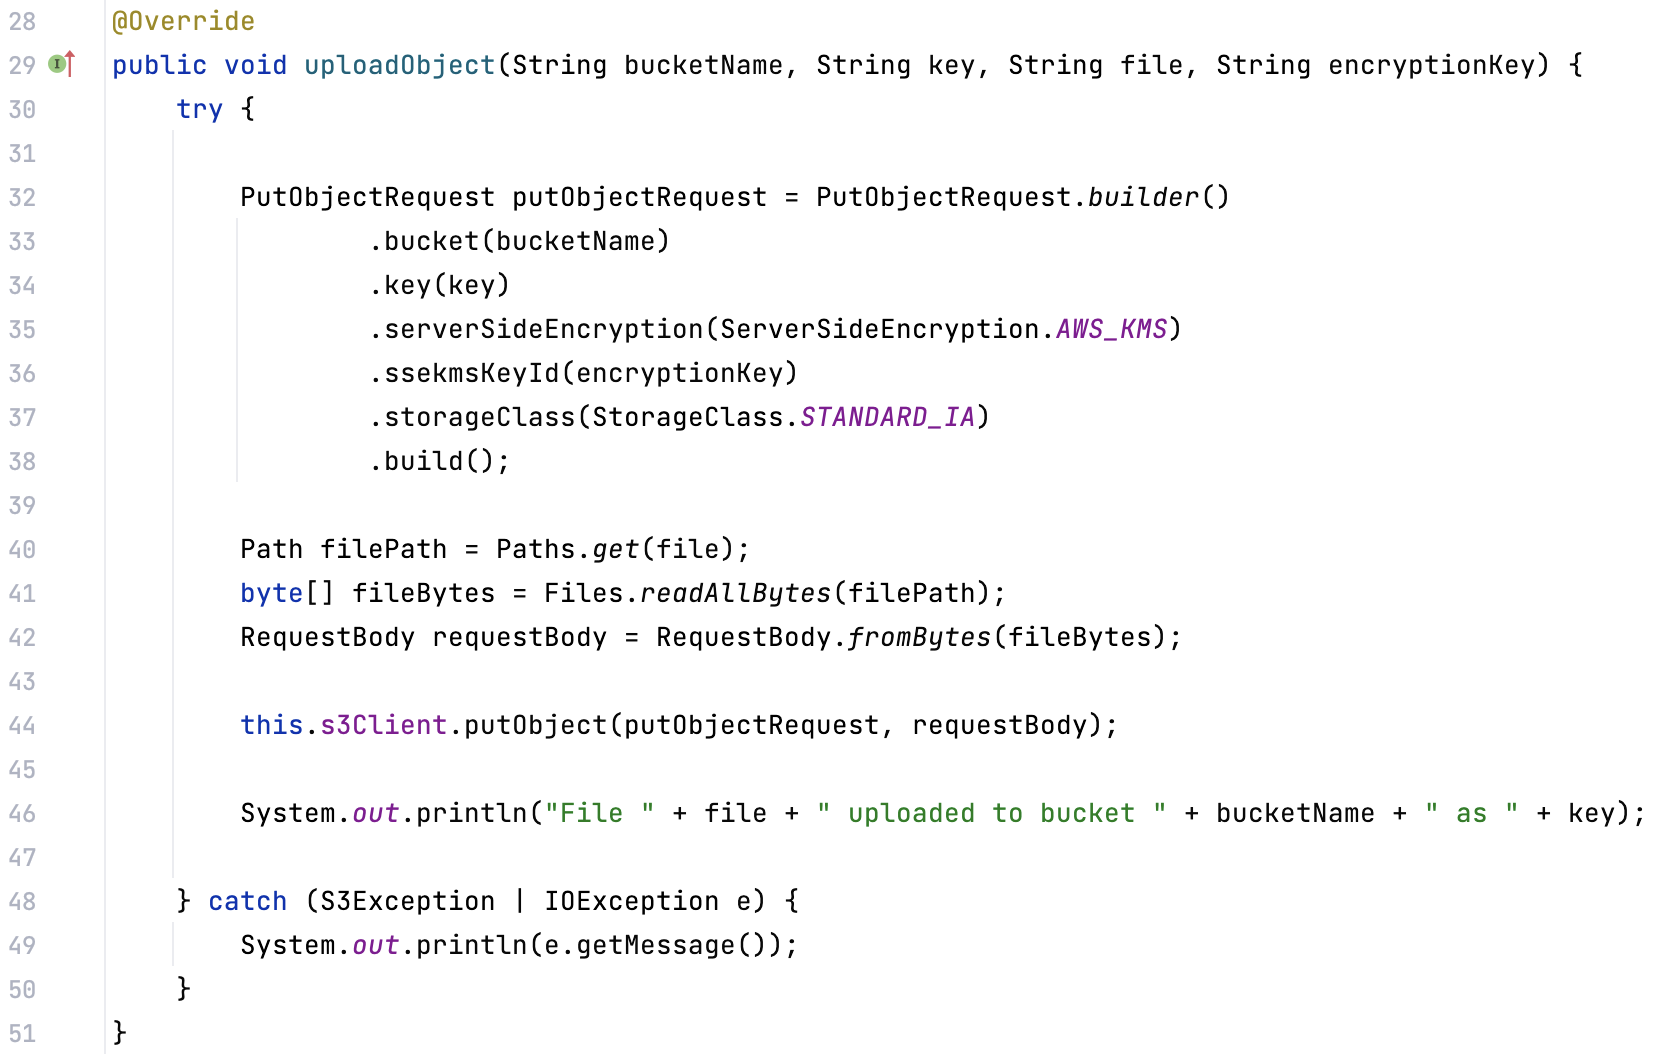
\includegraphics[width=15cm,keepaspectratio]{Pictures/UploadObjectAWS.png}
	\caption{Prototyp - Hochladen eines Objekts nach S3}
\end{figure}

\newpage

Der obere Code beschreibt den Speichervorgang eines Objekts nach AWS S3. Zuerst wird ein PUT Request Objekt erzeugt, indem die Parameter wie der Bucket Name, Objektname als Key und die Authentifizierungsmethoden angegeben werden. Es wird die AWS KMS Methode verwendet und den entsprechenden Schlüssel bereitgestellt. Zuletzt wird die Speicherklasse angegeben, indem das Objekt gespeichert wird. In diesem Beispiel wird die Standard - IA Klasse verwendet. Anschließend wird der Pfad der angegeben Datei gelesen, als Bytes Array umgewandelt und dem RequestBody übergeben. Dieser RequestBody gemeinsam mit dem PutObjectRequest wird an den S3Client übergeben und mit der AWS .putObject() Methode nach S3 hochgeladen. AWS S3 verschlüsselt das Objekt mit dem angegeben Encryption Key und ladet es nach S3 hoch.\\

Die folgenden Abbildung zeigt den Code Ausschnitt von der Klasse GoogleCloudStorageService. Ähnlich wie bei der Methode für AWS S3 wird auch hier ein Objekt nach Cloud Storage hochgeladen. 

\begin{figure}[h]
	\centering
	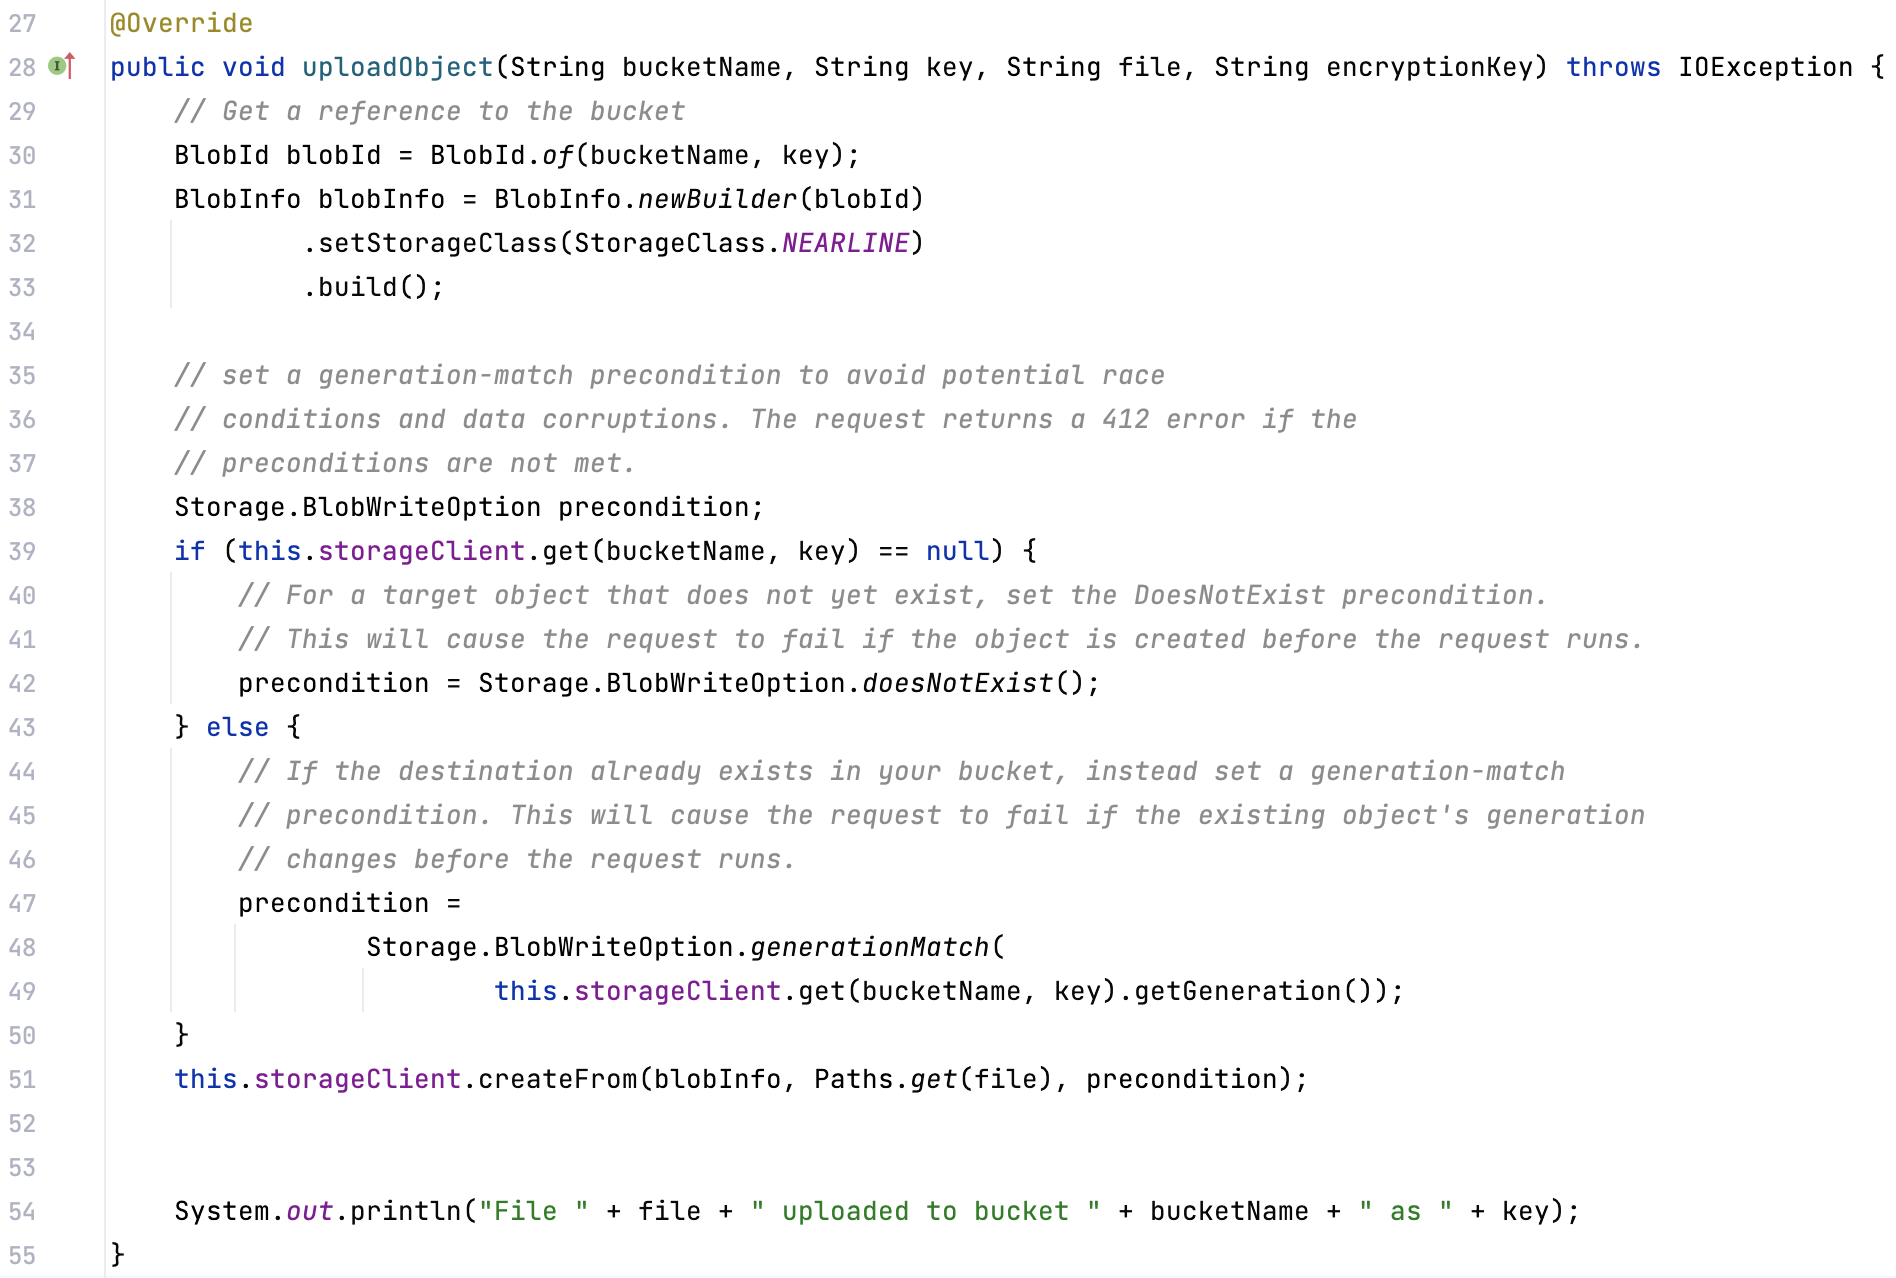
\includegraphics[width=15cm,keepaspectratio]{Pictures/UploadObjectGC.png}
	\caption{Prototyp - Hochladen des Objekt nach Cloud Storage}
\end{figure}

Dabei werden ähnliche Parameter der Methode wie in AWS S3 übergeben. Um ein Objekt in ein Bucket hochladen zu können, wird eine Referenz zum Bucket erstellt. Dies geschieht durch die BlobId, der den Bucket namen und den Namen des Objekts beinhaltet. Anschließend wird diese b†lobId dem BlobInfo Objekt übergeben und die Speicherklasse NEARLINE definiert. Anschließend wird über die Metadaten die KMS Encryption Key angegeben. Nach dem überprüft worden ist, ob das Objekt bereits im Bucket existiert oder nicht, wird das Objekt in der Zeile 58 hochgeladen.

Um das Programm zum Laufen zu bringen, wird die Hauptklasse \textbf{HandsonAwsGcApplication} ausgeführt. Damit das Programm erfolgreich läuft, müssen die Environment Variablen im System exportiert werden. Alle Environment Variablen sind in der \glqq application.properties\grqq hinterlegt. Diese werden beim Start des Programms gelesen und angewendet. Außerdem müssen die AWS  und Google Cloud Credentials hinterlegt werden. Dies kann entweder über die AWS Toolkit Plugin gesteuert werden oder mit dem Befehl \glqq aws configure\grqq in der Kommandozeile. Für Google Cloud Credentials kann mit dem Befehl \glqq export GOOGLE\_APPLICATION\_CREDENTIALS=<service-account-json-file> der Service Account hinterlegt werden oder durch Ausführen des Befehls "gcloud auth application-default login\grqq in der Kommandozeile, was die Credentials lokal speichert und für ADC verwendet wird.

\newpage

\section{Bereitstellung der Binärdaten}

Bei der Bereitstellung der Binärdaten geht es dabei um die signed URL Methode, um in leoticket Dateien über Links an den Kunden bereitzustellen. Es werden Code Implementierungen von beiden Cloud Providern vorgestellt und erläutert.\\

Die untere Abbildung zeigt die Methode der Klasse \textbf{AWSS3StorageService}:

\begin{figure}[h]
	\centering
	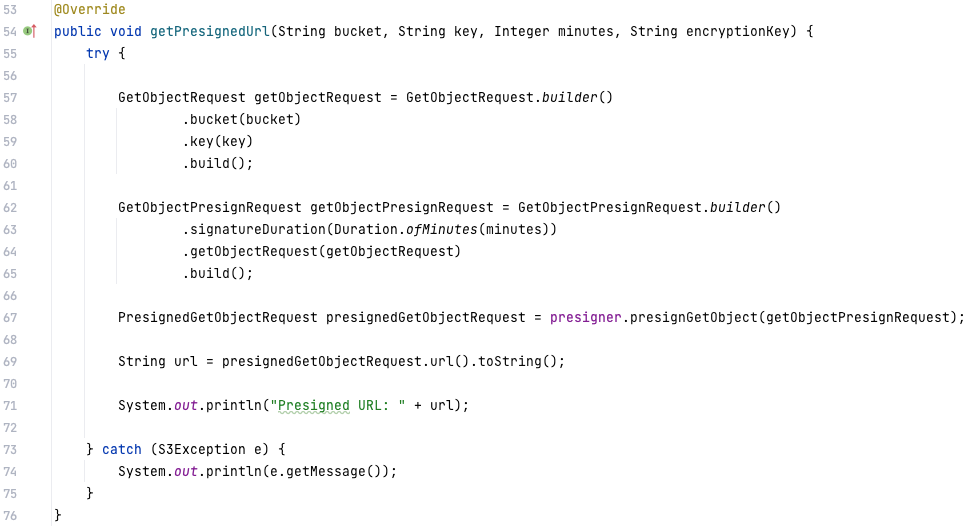
\includegraphics[width=13cm,keepaspectratio]{Pictures/AWSgetSignedUrl.png}
	\caption{Prototyp - AWS getPresignedUrl() Methode}
\end{figure}

Die Methode bekommt ähnlich wie beim Upload des Objekts erstmal die beiden Parameter Named des Bucket und Name des Objekts. Anschließend wird eine Zahl als Minuten übergeben, die dafür sorgt, dass der Link nur für diese bestimmte Zeit valide ist. Auch hier muss man den gleichen Encryption Key wie beim Upload für das Entschlüsseln der Daten mitgeben. In Zeile 57 wir das GetObjectRequest Objekt erstellt und den Bucket Namen und Objektnamen mitgegeben. Anschließend wird dieses Objekt dem GetObjectPresignRequest Objekt übergeben und dabei die Signaturdauer angegeben. Die Signaturdauer stellt die signierte URL solange wie die angegeben Minute zur Verfügung. Um nun die signierte URL zu erzeugen, wird die GetObjectPresignRequest dem S3Presigner übergeben, die presignGetObject() Methode darauf aufgerufen und dem PresignedGetObjectReuqest übergeben. In Zeile 69 wird die generierte URL als String gespeichert und anschließend ausgegeben.

\newpage

Bei der Methode von Cloud Storage ist der Vorgang zur Erstellung des signierten URLs kürzer. Folgende Abbildung zeigt die Methode zur Generierung des signierten URLs für Cloud Storage:

\begin{figure}[h]
	\centering
	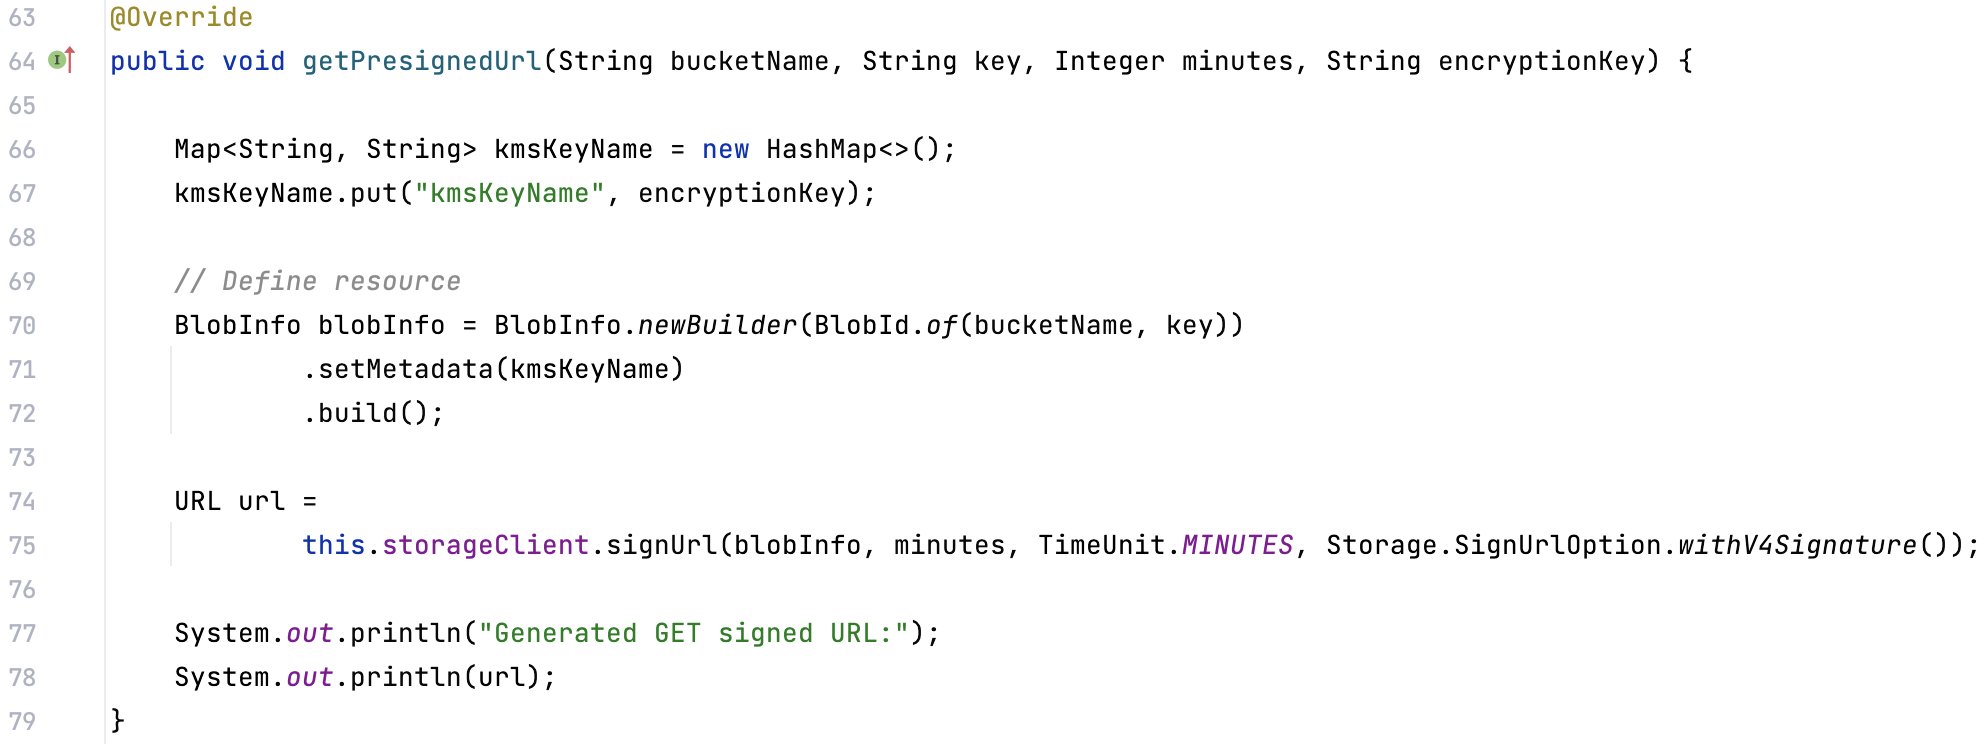
\includegraphics[width=12cm,keepaspectratio]{Pictures/GCgetSignedUrl.png}
	\caption{Prototyp - GC getPresignedUrl() Methode} 
\end{figure}

Ähnlich wie bei S3 wird eine Referenz zum Bucket erstellt, indem man den Bucket Namen und den Namen des Objekts dem BlobInfo Objekt mitgibt. Anschließend kann die URL durch Aufrufen der Methode in Zeile 63 erstellt werden. Hier wird das BlobInfo Objekt, die Minuten in und die Signatur Methode übergeben. Zuletzt wird die URL in der Kommandozeile ausgegeben.\\

Mit signierten URLs können die Anforderungen von leoticket an die sichere Speicherung und Bereitstellung der Daten über signierte URLs berücksichtigt werden. Dies bedeutet, Kunden können über diese Links die Dateien für Tickets und Rechnungen herunterladen ohne das Problem von zu großen Email-Anhängen zu haben.\\

\newpage

\section{Messung der Performance}

In diesem Abschnitt erfolgt die Messung der Performance für die Dienste von AWS und Google Cloud. Dabei werden bis zu 1000 generierte Dateien sowohl für den Upload als auch für den Download betrachtet.Die Performance Analyse wird auf einer virtuellen Maschine ausgeführt, um eine realistische Messung zu gewährleisten. Die Performancemessung beim Hoch- und Herunterladen kann jedoch von verschiedenen Faktoren wie Netzwerklatenz, verfügbarer Bandbreite, Serverkapazität, Datenmenge und der Auslastung der Server beeinflusst werden. Die Messungen dienen lediglich des groben Vergleichs beider Cloud Provider. Die Performance-Messung wird auf verschiedene Speicherklassen durchgeführt, um einen Vergleich zwischen dieser zu ermöglichen und eine Grundlage für die Bewertung ihrer Leistungsfähigkeit zu schaffen.\\


\textbf{AWS}\\

AWS bietet Dienste für die Performance Analyse. Unter anderem die Amazon CloudWatch, S3 Storage Lens und die S3 Transfer Acceleration. Die AWS CLI stellt einfache Methoden zum S3 Upload und Download Tests vor. Beispielsweise kann man mit dem Befehl:

%TODO Transfer Acceleration - kann beim Transfer von sehr großen Daten benutzt werden. Link zur Website https://s3-accelerate-speedtest.s3-accelerate.amazonaws.com/en/accelerate-speed-comparsion.html. 19% Schnellere Übertragung aber Gebühren.

\begin{code} aws s3 cp <lokaler_pfad> s3://<Bucket_Name>/<Ziel_Dateipfad>\end{code}

Dateien hoch,-und herunterladen und die Zeit für die benötigte Request verwenden. Auch mit der AWS SDK können Performance Test Skripte geschrieben werden. Diese Methode wird für den Prototypen angewendet. Dabei werden Tests bereitgestellt, die mehrere Dateien automatisch hoch, und herunterlädt und dabei die Zeit misst, die vergangen ist. 

\newpage

\textbf{Google Cloud Storage}\\

GC bietet einen eigenen "gsutil" Tool für die Performance Analyse. Im Abschnitt Performance bereits erwähnt können durch die perfdiag Funktion Performance Diagnosen erstellt werden. 

\begin{quote}
	Mehrere Testdateien werden aus einem angegebenen Bucket hoch-und heruntergeladen. Nach der Analyse werden alle Testdateien wieder gelöscht nach erfolgreicher Diagnose. Die gsutil Performance kann von einigen Fakoren beeinflusst werden wie vom Client, Server oder Netzwerk. Möglich sind die CPU Geschwindigkeit, der verfügbare Speicher, die Netzwerk Bandbreite, Firewalls und Fehlerraten zwischen gsutil und den Google Servern. Die perfiag Funktion wurde dafür bereitgestellt, damit Nutzer Messungen durchführen können, die beim Troubleshooting von Performance Problemen helfen, vgl. \cite{gc-perfdiag}.
\end{quote}

Um die Performance Diagnose auszuführen, kann der folgende Befehl verwendet werden:

\begin{code} gsutil perfdiag -o test.json -n 67000 -s 400kb gs://leoticket-bucket \end{code}

Die -o Option schreibt den Output des Ergebnisses in eine Datei. Die Output Datei ist eine JSON Datei mit System Informationen und enthält die Performance Diagnose Ergebnisse. Die -n Option setzt die Anzahl der Objekte, die heruntergeladen und hochgeladen werden sollen während dem Test. Mit der -s Option kann man die Objektgröße in bytes angeben. Zum Schluss wird der Name des Buckets angegeben. Damit der Befehl erfolgreich ausgeführt werden kann, braucht man die entsprechenden Rechte und muss sich authentifizieren können.\\

Um die Performance der SDKs zu analysieren, werden Objekte mit jeweils 100kb Objektgröße in verschiedenen Speicherklassen hoch-, und heruntergeladen. Anschließend wird die Performance über die SDK von Cloud Storage ähnlich wie bei AWS getestet. Der Test wird auf einer virtuellen Maschine ausgeführt.\\

Die Performance wird schrittweise gemessen. Angefangen von einer Datei bis hin zu 1000 Dateien in 10-fach Schritten. Das bedeutet, es werden die Messsungen für eine Datei, für zehn Dateien, für 100 Dateien und für 1000 Dateien untersucht. Um die Messung durchzuführen, wird eine Java Jar Datei des Prototyps erstellt. Dabei werden die Testmethoden ausgeführt. Die Testmethoden generieren zuerst die Testdaten gefüllt mit zufälligen String Werten in der Größe von 100kb. Anschließend werden die Testmethoden in der Kommandozeile ausgeführt.

\newpage

\subsection{Messungsergebnisse}

In diesem Abschnitt werden die Messungsergebnisse der Performance Messung in genauen Zahlen in Millisekunden bereitgestellt. Die Speicherklassen Standard, Standard-IA und One Zone-IA von AWS wurden jeweils mit Standard, Nearline und Coldline von GC gemessen und verglichen. Im folgenden werden die Ergebnisse der Upload und Download Geschwindigkeit aller Speicherklassen präsentiert: Test

\begin{code}
STANDARD-IA vs. NEARLINE

1 File---------------------------------------------------------------------------

Elapsed Time for 1  Object Upload in S3:-------------------------------705ms.
Elapsed Time for 1 Object Upload in Cloud Storage:---------------------841ms.

Elapsed Time for 1 Object Download in S3:------------------------------18ms.
Elapsed Time for 1 Object Download in Cloud Storage:-------------------26ms.

10 Files-------------------------------------------------------------------------

Elapsed Time for 10  Object Uploads in S3:-----------------------------1862ms.
Elapsed Time for 10 Object Uploads in Cloud Storage:-------------------3217ms.

Elapsed Time for 10 Object Downloads in S3:-----------------------------35ms.
Elapsed Time for 10 Object Downloads in Cloud Storage:------------------94ms.

100 Files------------------------------------------------------------------------

Elapsed Time for 100  Object Uploads in S3:-----------------------------16681ms.
Elapsed Time for 100 Object Uploads in Cloud Storage:-------------------22683ms.

Elapsed Time for 100 Object Downloads in S3:----------------------------129ms.
Elapsed Time for 100 Object Downloads in Cloud Storage:-----------------269ms.

1000 Files-----------------------------------------------------------------------

Elapsed Time for 1000  Object Uploads in S3:----------------------------71175ms.
Elapsed Time for 1000 Object Uploads in Cloud Storage:------------------1851348ms.

Elapsed Time for 1000 Object Downloads in S3:---------------------------663ms.
Elapsed Time for 1000 Object Downloads in Cloud Storage:----------------1489ms.
\end{code}

\newpage

\begin{code}
STANDARD vs. STANDARD

1 File---------------------------------------------------------------------------

Elapsed Time for 1  Object Upload in S3:--------------------------------585ms.
Elapsed Time for 1 Object Upload in Cloud Storage:----------------------660ms.

Elapsed Time for 1 Object Download in S3:-------------------------------28ms.
Elapsed Time for 1 Object Download in Cloud Storage:--------------------19ms.

10 Files-------------------------------------------------------------------------

Elapsed Time for 10  Object Uploads in S3:------------------------------1369ms.
Elapsed Time for 10 Object Uploads in Cloud Storage:--------------------3002ms.

Elapsed Time for 10 Object Downloads in S3:-----------------------------70ms.
Elapsed Time for 10 Object Downloads in Cloud Storage:------------------108ms.

100 Files------------------------------------------------------------------------

Elapsed Time for 100  Object Uploads in S3:-----------------------------8110ms.
Elapsed Time for 100 Object Uploads in Cloud Storage:-------------------20750ms.

Elapsed Time for 100 Object Downloads in S3:----------------------------180ms.
Elapsed Time for 100 Object Downloads in Cloud Storage:-----------------396ms.

1000 Files-----------------------------------------------------------------------

Elapsed Time for 1000  Object Uploads in S3:----------------------------73992ms.
Elapsed Time for 1000 Object Uploads in Cloud Storage:------------------176004ms.

Elapsed Time for 1000 Object Downloads in S3:---------------------------650ms.
Elapsed Time for 1000 Object Downloads in Cloud Storage:----------------1619ms.

\end{code}

\newpage

\begin{code}
ONEZONE-IA vs. COLDLINE

1 File---------------------------------------------------------------------------

Elapsed Time for 1  Object Upload in S3:--------------------------------505ms.
Elapsed Time for 1 Object Upload in Cloud Storage:----------------------636ms.

Elapsed Time for 1 Object Download in S3:------------------------------28ms.
Elapsed Time for 1 Object Download in Cloud Storage:-------------------18ms.

10 Files-------------------------------------------------------------------------

Elapsed Time for 10  Object Uploads in S3:------------------------------1105ms.
Elapsed Time for 10 Object Uploads in Cloud Storage:--------------------2855ms.

Elapsed Time for 10 Object Downloads in S3:-----------------------------65ms.
Elapsed Time for 10 Object Downloads in Cloud Storage:------------------89ms.

100 Files------------------------------------------------------------------------

Elapsed Time for 100  Object Uploads in S3:-----------------------------7539ms.
Elapsed Time for 100 Object Uploads in Cloud Storage:-------------------20391ms.

Elapsed Time for 100 Object Downloads in S3:----------------------------187ms.
Elapsed Time for 100 Object Downloads in Cloud Storage:-----------------250ms.

1000 Files-----------------------------------------------------------------------

Elapsed Time for 1000  Object Uploads in S3:----------------------------73086ms.
Elapsed Time for 1000 Object Uploads in Cloud Storage:------------------163661ms.

Elapsed Time for 1000 Object Downloads in S3:---------------------------701ms.
Elapsed Time for 1000 Object Downloads in Cloud Storage:----------------1559ms.
\end{code}


Die Ergebnisse werden im Kapitel Zusammenfassung der Ergebnisse zusammengefasst und als Liniendiagramm dargestellt.

\newpage

\section{Zusammenfassung der Implementierung}

Der Prototyp soll einen Vergleich zwischen den beiden Cloud Providern bieten. Das Ziel dabei ist es, ähnliche Technologien von beiden Providern zu verwenden und die Performance mit Testdaten dabei messen zu können. Es dient für zwei Funktionen. Das Hochladen und Herunterladen von Dateien. Dabei werden die Anforderungen an leoticket mitberücksichtigt. Das bedeutet, das signierte URLs für die Bereitstellung der Dateien verwendet werden. Außerdem wird für die Datenverschlüsselung die SSE KMS von beiden Providern angewendet. Außerdem soll der Prototyp im weiteren Verlauf als externe Library für eigene Anwendungen integriert werden. Für die Implementierung wurden die offiziellen Dokumentationen von AWS und GC verwendet, um die aktuellsten Versionen zum Zeitpunkt der Arbeit bereitzustellen. Des weiteren wurde auf Wunsch von Leomedia Spring Boot als Framework verwendet, um eine Enterprise Anwendung bereitstellen zu können. Terraform wird dabei für die Erstellung von Buckets erstellt und stellt auch ein Vergleich für die Integration der beiden Providern nach Terraform dar. Aus Preferenzgründen wird Java als Programmiersprache gewählt, jedoch stellen beide Provider viele weitere Sprachen, die bereits im Kapitel API Anbindung erwähnt wurden, zur Verfügung.\\

Der Prototyp wurde so aufgebaut, dass man zwischen AWS und GC durch eine Environment Variable wählen kann. Die Klasse \textbf{CloudStorageServiceFactory} stellt die Auswahl zwischen AWS und GC zur Verfügung. Je nachdem welchen Cloud Provider der Nutzer angegeben hat, wird die entsprechende Klasse instanziiert und aufgerufen. Die Klassen \textbf{AWSS3StorageService} und \textbf{GoogleCloudStorageService} implementieren die Methoden des Interfaces \textbf{CloudStorageService}.\\

Die bereitgestellten Tests dienen der Performance Messung. Dabei werden Dateien automatisch als 400kb große Objekte erstellt und durch die Testmethoden verwendet, um Objekte hoch-, und herunterzuladen. Sie unterstützen dabei, die Geschwindigkeit der verschiedenen Funktionen zu messen.\\

Da die Maven Dependencies kein Teil der Spring Cloud Release Train sind, hängt es von der Commmunity ab, die Versionen aktuell zu halten. Für AWS bedeutet dies, dass die AWS SDK 2. Version nicht komplett abgedeckt ist. Jedoch ist sie so weit, dass S3 bereits unterstützt wird. 

